\documentclass[10pt,twocolumn,letterpaper]{article}

\usepackage{cvpr}
\usepackage{times}
\usepackage{epsfig}
\usepackage{graphicx}
\graphicspath{./img}
\usepackage{amsmath}
\usepackage{amssymb,bbm,xcolor}
\usepackage[breaklinks=true,bookmarks=false]{hyperref}
\usepackage{lipsum}
\usepackage{listings}
\usepackage{mathtools,eucal}
\usepackage{graphicx}

\usepackage{bbold}
\usepackage{caption}
\usepackage{subcaption}
\usepackage{algorithm}
\usepackage[noend]{algpseudocode}
\usepackage{booktabs, multicol, xcolor}
\usepackage[shortlabels]{enumitem}
\usepackage{changepage}
\cvprfinalcopy % *** Uncomment this line for the final submission
\setcounter{page}{1}
\renewcommand{\figurename}{Figure}
\usepackage{amsmath}
\DeclareMathOperator*{\argmax}{arg\,max}
\DeclareMathOperator*{\argmin}{arg\,min}
\DeclareMathAlphabet\mathbfcal{OMS}{cmsy}{b}{n}
\usepackage[T1]{fontenc}
\usepackage{flushend}

% Include other packages here, before hyperref.

% If you comment hyperref and then uncomment it, you should delete
% egpaper.aux before re-running latex.  (Or just hit 'q' on the first latex
% run, let it finish, and you should be clear).
\usepackage[breaklinks=true,bookmarks=false]{hyperref}

\cvprfinalcopy % *** Uncomment this line for the final submission

% Pages are numbered in submission mode, and unnumbered in camera-ready
%\ifcvprfinal\pagestyle{empty}\fi
\setcounter{page}{1}

\begin{document}
\title{Automatic image colorization: a comparative overview}
\author{Bigarella Chiara\\
{\tt\small Student nr. 2004248}
% For a paper whose authors are all at the same institution,
% omit the following lines up until the closing ``}''.
% Additional authors and addresses can be added with ``\and'',
% just like the second author.
% To save space, use either the email address or home page, not both
\and
Poletti Silvia\\
{\tt\small Student nr. 1239133}
}

\maketitle
%\thispagestyle{empty}

%%%%%%%%% ABSTRACT
\begin{abstract}
   The ABSTRACT is to be in fully-justified italicized text, at the top
   of the left-hand column, below the author and affiliation
   information. Use the word ``Abstract'' as the title, in 12-point
   Times, boldface type, centered relative to the column, initially
   capitalized. The abstract is to be in 10-point, single-spaced type.
   Leave two blank lines after the Abstract, then begin the main text.
   Abstract should be no longer than 300 words.
\end{abstract}

\section{Introduction}
Introduction (10\%): describe the problem you are working on, why it's important, and an overview of your results

\section{Related Work}
Related Work (10\%): discuss published work or similar apps that relates to your project. How is your approach similar or different from others?

Papers are: \cite{chromagan}, \cite{su}, \cite{zhang},\cite{siggraph}, \cite{dahl},\cite{animation},\cite{cartoonize},\cite{language}.

\section{Dataset}
We considered three types of images: 4023 originally colored images from five different datasets, 18 originally black and white images from various artists and 180 filtered images (see more details in Experiments section) obtained starting from 18 originally colored images.

Indeed, our data includes heterogeneous images, representing many different environments, situations and subjects.
For what concerns the originally colored images, we considered various sources:
\begin{itemize}
	\item subset of ImageNet made of 12 classes (200 images each) taken from \cite{imagenette}, ten of which are easily classified classes (tench, English springer, cassette player, chain saw, church, French horn, garbage truck, gas pump, golf ball and parachute) while the other two are not so easy to classify (Samoyed and Rhodesian ridgeback);
	\item subset of 100 randomly selected images from Pascal VOC \cite{pascal} representing realistic scenes in which the subjects could be animals, human beeings, plants, rooms, landscapes, various objects and vehicles;
	\item subset of 200 randomly selected images form Places205 \cite{place} reguarding mountain, desert, sea, beach and island landscapes.
	\item subset of 325 Bird Species \cite{bird} made of 8 classes (100 images each), which were selected to depict those birds having the most unusual colors (Cuban Tody, Fire Tailed Myzornis, Flamingo, Nicobar Pigeon and Pink Robin) and those that are well-known by the majority of people (Bald Eagle, Ostrich and Touchan);
	\item subset of 102 Category Flowers \cite{flower} made of 6 classes (from 50 to 100 images each), which were selected to depict those flowers having the most unusual colors and shapes (Purple Coneflower, Grape Hyacinth, Hibiscus) and those that are well-known by the majority of people (Rose, Water Lily and Giant White Arum Lily).
\end{itemize}

The images have been treated by using OpenCV (ChromaGAN and InstColorization) or Pillow combined with Skimage (Baseline, Dahl, Zhang, Siggraph).

The images have been reshaped to various formats ($256\times256\times3$ for Baseline, Zhang, Siggraph and InstColorization and $224\times224\times3$ for Dahl and ChromaGAN) and Dahl also required center cropping and desaturation. Despite the preliminar reshape, Zhang, Siggraph and Chromagan models are built in a way that allows to obtain colorized images having the original shape.

Given an RGB image (additive colour model in which red, green and blue primary colour channels are added together) we obtain the corrisponding image in the \textit{Lab} color space, in which colors are expressed through 3 new channels: $L$ for perceptual lightness ($L=0$ corresponds to white, $L=100$ corresponds to black), $a$ and $b$ for four primary colors ($a=\pm100$ correspond to red and green, $b=\pm100$ correspond to yellow and blue).

Our models get only the $L$ channel as input (greyscale images) with the goal of predicting the $a$ and $b$ channels. Then, the resulting images are projected again in the RGB color space.

Moreover, the classification with AlexNet required the normalization of the images' RGB channels in the range $[0,1]$ and a further standardization of the images according to the mean and standard deviation of the training set images. 

On the other hand, the LPIPS metric required the normalization of the images' RGB channels in the range $[-1,1]$ and the dataset reshaping from $N\times H\times W\times3$ to $N\times3\times H\times W$, where $N$ is the number of images.

\section{Methods}
In order to carry out a comparative overview about automatic image colorization, we built, trained and tested a simple autoencoder based on cartoonization, to be considered as baseline. Then, we tested some state-of-the-art pre-trained models taken from the literature: Dahl, Zhang and its upgraded version Siggraph, ChromaGAN and InstColorization.

\subsection{Baseline}
As a baseline, we built with Keras a simple autoencoder having 8 Convolutional layers for the encoding part (ReLU activations, zero-padding, $3\times3$ kernels and sometimes $2\times2$ strides), while the decoding part consisted in a combination of 5 Convolutional layers (relu activations except for the last layer, zero-padding and $3\times3$ kernel) and 3 UpSampling layers of size $2\times2$. The encoder learns a compact representation of the black and white input image and the decoder generates the corresponding novel coloured image.

The model was trained (50 epochs) on a heterogeneous dataset containing all the data available.

Moreover, we enriched this model with a novel approach: instead of using the original dataset, we fed the model with the cartoonized (black and white) version of the images, computed with the pre-trained GAN cartoonization model by \cite{cartoonize}. This cartoonization provides fine-grained results (we don't miss much information) and synthesizes the original images in order to exclude noisy elements that could interfer with the colorization task. The model produces cartoonized colored images whose $a$ and $b$ channels are combined with the $L$ channel of the original \textit{Lab} images. Therefore, we mantain the original details of the pictures, while producing a more precise and sectorial colorization.

For comparison, we also include in our experiments the Baseline without cartoonization (Baseline w/c).
\subsection{Dahl}

Dahl's model is an autoencoder from black and white images to colored ones, with
residuals connections.
As shown in Figure \ref{fig:dahl}, the encoder is a VGG-16 network with ReLUs as activation functions, that takes in input greyscale images and infers
some color information at each layer. This information is added up in the decoder thanks to the residual
connections, until a 224 x 224 x 3 tensor is constructed. In the last layer of the decoder, a sigmoid activation
function is used to squash the values between 0 and 1.
Finally, the model's loss function is the average of the following three Euclidean Distances:
\begin{itemize}
    \item the Euclidean Distance computed between the original colored image and the network output;
    \item the Euclidean Distance computed between the original colored image and the network output, blurred with a 3 pixel gaussian kernel;
    \item the Euclidean Distance computed between the original colored image and the network output, blurred with a 5 pixel gaussian kernel.
\end{itemize}

Differently to the other models, Dahl's model uses the YUV color encoding system which consists of one luma
component (Y) and two chrominance components, called U (blue projection) and V (red projection) respectively.

One of the biggest disadvantage of this model is the fact that it handles 224 x 224 images only. This means that
bigger images have to be cropped and reshaped during the preprocessing, leading to some information loss.

% It has been trained on the ILSVRC 2012 classification training dataset.


\subsection{Eccv16}
The innovation introduced by Zhang's colorization model is not the model's architecture (a CNN made of 8 blocks of
two or three repeated Convolutional and ReLU layers followed by a BatchNorm layer, as shown in Figure \ref{fig:zh}) but rather a more suitable loss function for saturated colorization, combined with class rebalancing, which allows to increase the diversity of colors in the results.

Since an object can potentially have several plausible colorization, the model accounts for the multimodal
distribution of possible colors for each pixel. The intrinsic multimodal nature of the colorization
problem can't be captured by a simple Euclidean loss between the target and the predicted colors. Instead, the
model learns a map $\mathcal{G}: \mathbb{R}^{H\times W\times1}\rightarrow [0,1]^{H\times W\times Q}$ from the grayscale input to a probability
distribution $\hat{Z}=P(a,b)$ over $Q=313$ possible $(a,b)$ pairs (i.e. colors), which were obtained through the
quantization of the \textit{ab} output space, as shown in Figure \ref{fig:q}. Then, the multimomial crossentropy
los is defined as:

\begin{equation*}
	\mathcal{L}_{cl} (\hat{Z},Z)= - \sum_{h,w} v(Z_{h,w})\sum_q Z_{h,w,q}log(\hat{Z}_{h,w,q})
\end{equation*}
where $Z$ is the soft-encoded target (obtained by taking the 5-nearest neighbors in the quantized \textit{ab} space
for each groundtruth pixel, and weighting them according to their distance from the groundtruth) and $v$ is a
weighting function for class rebalancing, in order to emphasize rare colors.

To conclude, the final predicted colorization $\hat{Y}$ is the annealed-mean of the distribution $\hat{Z}$, which
consists in taking the mean of the softmax distribution $\sigma_T(\hat{Z}) = \sigma(\hat{Z}/T)$ adjusted according the
temperature parameter T. This avoids desaturated or spatially inconsistent results.
\subsection{Chromagan}


\subsection{InstColorization}
Instead of just performing learning and colorization on the entire image, InstColorization learns meaningful object-level semantics within the bounding boxes localized by an object detector. Then, we have two colorization networks: the first colorizes the whole image and the second the patches (resized to $256\times265$) in the bounding boxes. These networks have different weights but share the same architecture: the chosen architecture is the same as Zhang, as well as the loss function. Once the first networks is trained, its learned weights are used to inizialize the second network. At the end of the second network's training, the resulting full-image features and object-level features have to be combined in a consistent way by a fusion module. This allows to obtain better results on scenes with multiple objects in a cluttered background. The whole process is reported in Figure \ref{fig:su1}.

In particular, the fusion module (Figure \ref{fig:su2}) takes place at multiple layers of the colorization networks. For each layer, the full-image feature and the $N$ object-level features ($N$ is the number of detected objects) are processed by a small CNN and then combined by taking the weighted sum of the stack composed by the full-image weight map and the patches' weight maps, which have been previously reshaped (and zero padded) using the size and location of the bounding boxes for each object.




\section{Experiments}
To compare the results of each model, we computed several metrics: classification with AlexNet, LPIPS, PSNR and SSIM (all quantitative metrics) and a Turing test on few images (qualitative metric). Finally, we applied image filtering to evaluate possible improvements in the performances.

\subsection{Classification with AlexNet}
First, we considered the AlexNet classifier pre-trained on ImageNet and tested on the ImageNet subset in its original, black and white and re-colorized versions.

\begin{table*}[ht]
	\begin{center}
		\begin{adjustwidth}{-1cm}{}
			\begin{tabular}{c|ccccccccc}
				&\textbf{Original} & \textbf{B\&W} & \textbf{Baseline w/c}&\textbf{Baseline} & \textbf{Dahl} & \textbf{Eccv16} & \textbf{Siggraph17} & \textbf{ChromaGAN} & \textbf{InstColorization}  \\
				\midrule
				\textbf{Pre-trained} & 74.5\% & 43.1\% & 32.5\% & 34.0\% & 39.8\% & 42.7\% & 43.2\% & 46.8\% & 49.5\% \\
				\midrule
				\textbf{Feature Extraction} & 97.2\% & 84.2\% & 79.4\% & 80.4\% & 87.8\% & 87.6\% &  88.9\%   &  90.2\% &       90.0\% \\
				\midrule
				\textbf{Finetuning} & 99.7\% & 63.0\% & 58.4\% & 63.6\% & 64.4\% & 80.9\% &  79.9\%   &  77.9\% &       73.7\% \\
			\end{tabular}
		\end{adjustwidth}
	\end{center}
	\caption{{\small  Summary of the classification accuracy of Alexnet in three different settings: Alexnet pre-trained on Imagenet, Alexnet feature extraction for the ImageNet subset, AlexNet finetuning for the Birds and Flowers dataset.}}
	\label{tab:pre-trained}
\end{table*}

\begin{figure*}[t]
	\centering
	\captionsetup[subfigure]{labelformat=empty}
	\begin{subfigure}[b]{0.1\textwidth}
		\centering
		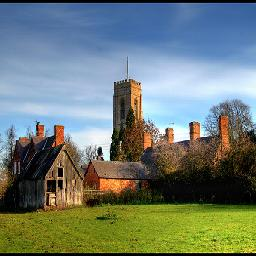
\includegraphics[width=2cm]{or - imgnet.jpeg}
	\end{subfigure}
	\hfill
	\begin{subfigure}[b]{0.1\textwidth}
		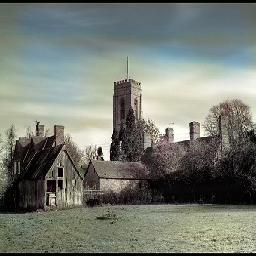
\includegraphics[width=2cm]{b - imgnet.jpeg}
	\end{subfigure}
	\hfill
	\begin{subfigure}[b]{0.1\textwidth}
		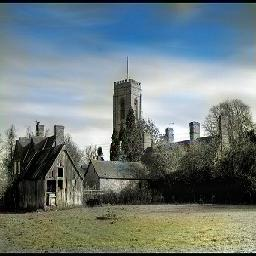
\includegraphics[width=2cm]{bw - imgnet.jpeg}
	\end{subfigure}
	\hfill
	\begin{subfigure}[b]{0.1\textwidth}
		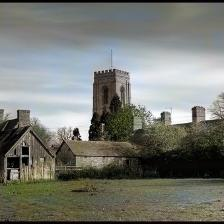
\includegraphics[width=2cm]{d - imgnet.jpeg}
	\end{subfigure}
	\hfill
	\begin{subfigure}[b]{0.1\textwidth}
		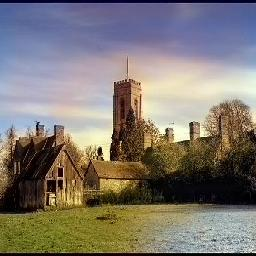
\includegraphics[width=2cm]{z - imgnet2.jpeg}
	\end{subfigure}
	\hfill
	\begin{subfigure}[b]{0.1\textwidth}
		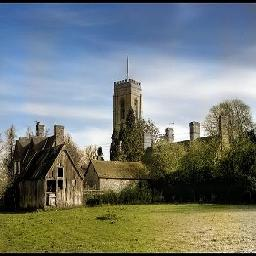
\includegraphics[width=2cm]{si - imgnet2.jpeg}
	\end{subfigure}
	\hfill
	\begin{subfigure}[b]{0.1\textwidth}
		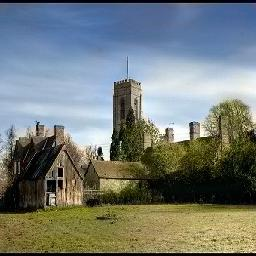
\includegraphics[width=2cm]{chr - imgnet2.jpeg}
	\end{subfigure}
	\hfill
	\begin{subfigure}[b]{0.1\textwidth}
		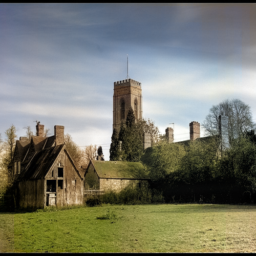
\includegraphics[width=2cm]{su - imgnet.png}
	\end{subfigure}

	\vspace{0.1cm}
	\begin{subfigure}[b]{0.1\textwidth}
		\centering
		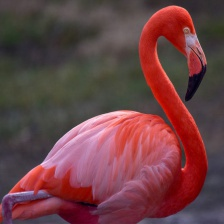
\includegraphics[width=2cm]{or - flamingo.jpg}
		\caption{Original}
	\end{subfigure}
	\hfill
	\begin{subfigure}[b]{0.1\textwidth}
		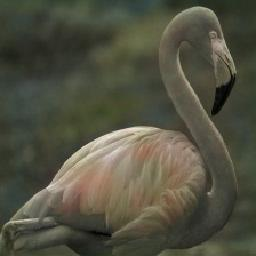
\includegraphics[width=2cm]{bw - flamingo.jpg}
		\caption{Baseline w/c}
	\end{subfigure}
	\hfill
	\begin{subfigure}[b]{0.1\textwidth}
		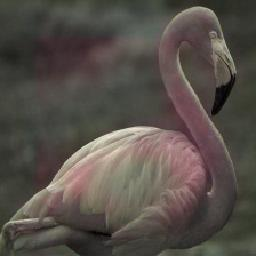
\includegraphics[width=2cm]{b - flamingo.jpg}
		\caption{Baseline}
	\end{subfigure}
	\hfill
	\begin{subfigure}[b]{0.1\textwidth}
		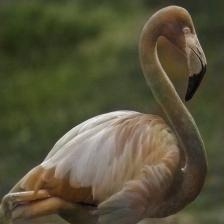
\includegraphics[width=2cm]{d - flamingo.jpg}
		\caption{Dahl}
	\end{subfigure}
	\hfill
	\begin{subfigure}[b]{0.1\textwidth}
		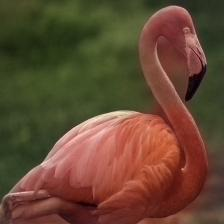
\includegraphics[width=2cm]{z - flamingo.jpg}
		\caption{Eccv16}
	\end{subfigure}
	\hfill
	\begin{subfigure}[b]{0.1\textwidth}
		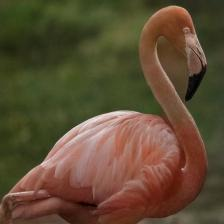
\includegraphics[width=2cm]{si- flamingo.jpg}
		\caption{Siggraph17}
	\end{subfigure}
	\hfill
	\begin{subfigure}[b]{0.1\textwidth}
		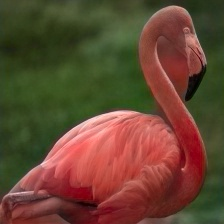
\includegraphics[width=2cm]{chr - flamingo.jpg}
		\caption{ChromaGAN}
	\end{subfigure}
	\hfill
	\begin{subfigure}[b]{0.1\textwidth}
		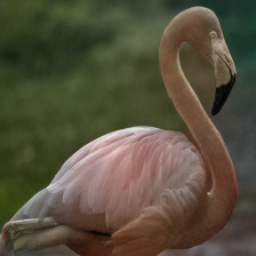
\includegraphics[width=2cm]{su - flamingo.png}
		\caption{InstColoriz.}
	\end{subfigure}
	\caption{{\small Colorization comparison on two images from ImageNet Church (first row) and Bird Species Flamingo (second row).}}
	\label{fig:imagenet}
\end{figure*}

Table \ref{tab:pre-trained} reports the AlexNet classification accuracy in this setting and in other two settings that we will discuss later in this section. Note that the Baseline without cartoonization (Baseline w/c) always reaches a slightly worse accuracy than the Baseline combined with cartoonization, meaning that our approach is valid and can actually improve the colorization performance.

The great gap in the accuracies computed on the original and the black and white versions of the images suggests that colors play an important role in image classification.

The best colorizations according to this experiment are given by ChromaGAN and InstColorization, while the Baseline and Dahl are not even able to improve the accuracy with respect to the black and white images.\\

Overall, the accuracy on the models' colorizations is much lower than the one computed on the original images and the latter is relatively low. Therefore we applied feature extraction to better focus on our ImageNet subset: we used the pre-trained AlexNet as a fixed feature-extractor, and only updated the final layer (for 2 epochs) in order to consider just our 12 ImageNet classes. This resulted in more reliable accuracy values and all the models except the Baseline are able to outperform the black and white images.\\

For a further comparison, we applied finetuning to perform classification on the birds and flowers images, which present more vibrant and various colors than our ImageNet subset: we updated (for 2 epochs) all the AlexNet parameters for the new task. In this new setting we have, as expected, a greater gap than before between the original and the black and white accuracies, meaning that the color is much more relevant. Indeed, all the models including the Baseline with cartoonization are able to improve the accuracy with respect to the black and white images.

The best colorizations according to this experiment are given by the Eccv16 and Siggraph17 models, which are able to generalize better across different datasets.

In this last setting, we can notice a general decreasing in the accuracy (except for the original images) with respect to the feature extraction using the ImageNet subset. This is due to the fact that our pre-trained models have been trained on Image-Net and their colorization of the birds and flowers images are overall bad. However, looking at our results, a badly colored image generally seems more distinguishable than its black and white version.

To conclude, the colorizations of two images are reported as an example in Figure \ref{fig:imagenet}.


\subsection{LPIPS, PSNR and SSIM Metrics}

\cite{psnr-ssim} and \cite{lpips}
\subsection{Turing Test}
The Turing test is a qualitative metric based on human perceptions. Due to our limited resources we just elaborate a short survey on Google Forms, divided into two sections: we asked the participants to first evaluate the colorizations of three black and white photographs and then evaluate the ri-colorizations of four originally colored images. 

A preliminary test has been conducted on a restricted sample of partecipants, who were always be able to dicriminate between the original version of the images and the ri-colorizations. Therefore, we decided to not show the original colored images in the final Turing test in order to avoid biases on the different and equally plausible choices of colors. 

The 124 participants had to score how realistic was each colorization in a
scale from 1 (not realistic at all) to 5 (very realistic). The test includes only the best colorizers, namely Eccv16, Siggraph17, ChromaGAN and InstColorization. Figure \ref{fig:turing} summarizes the mean scores for each model. Clearly, the models performed differently on originally colored images and greyscale photographs, since these ones have a low-level image statistics which are quite different from those of the modern-day photos on which the models were trained \cite{zhang}.
Overall, the best average scores are reached by Siggraph17 and ChromaGAN.

\begin{figure}[h]
	\centering
	\captionsetup[subfigure]{labelformat=empty}
	\begin{subfigure}[b]{0.1\textwidth}
		\begin{adjustwidth}{-1.1cm}{}
		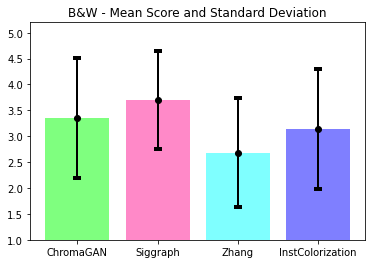
\includegraphics[width=4cm]{bw turing.png}
		\end{adjustwidth}
	\caption{B\&W}
	\end{subfigure}
\hspace{2.3cm}
	\begin{subfigure}[b]{0.1\textwidth}
		\begin{adjustwidth}{-1.1cm}{}
			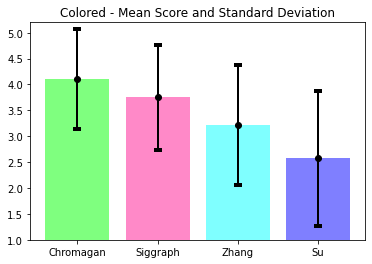
\includegraphics[width=4cm]{col turing.png}
		\end{adjustwidth}
		\caption{Colored}
	\end{subfigure}
	\caption{{\small Mean scores obtained with the colorization on black and white photographs and originally colored images.}}
	\label{fig:turing}
\end{figure}
\subsection{Image filtering}
\label{section:filtering}

Our last experiment consists in applying some filters to a selection of 18 ImageNet images to evaluate possible changes in the image colorization output. We considered a blurring filter with kernel sizes of 3, 7 or 11, a cartoonizing filter from \cite{cartoonize} and the increasing or decreasing of contrast and luminance.

In general, a blurred image is harder to colorize, and the more blurred the image is, the worse
the final colorization we get. Indeed, in the example reported Figure \ref{fig:filter} the dogs have some weird pink/orange
spots on their fur.
On the contrary, images with a higher contrast and luminance get a better colorization
by all the models, with just a few exceptions depending on the specific image.

Clearly, with cartoonization we reach very unrealistic colors. In the example, it looks like the model
didn't recognize the grass and probably mistook it for water. Probably, this is not due to the fact that cartoonization
discards some details from the original images, because blurring does the same. This could be rather due to the
fact that the models are not trained on cartoonized images and expect a completely different "image style" in input.

In conclusion, Figure \ref{fig:filter} is a good example of how the colorization is an ambiguous task: the model colors the grass with a plausible green tone, which actually could result more realistic than the original brown tone.



\section{Conclusion}
baseline fa schifo perchè l'architettura è piccola/semplice, non c'è una loss studiata apposta per image colorization, il training set è troppo piccolo e non abbastanza vario.


Conclusion (5\%): summarize your key results; what have you learned? Suggest ideas for future extensions.


{\small
\bibliographystyle{ieee_fullname}
\bibliography{egbib}
}

\end{document}
